%! TEX root = course_report.tex

\section{Проектирование графического пользовательского интерфейса} % (fold)
\label{sec:gui_design}


\subsection{Обоснование проекта пользовательского интерфейса}
\label{sub:gui_design:motivation}

Для получения эффективного результата разработки интерфейса используют различные подходы к проектированию:

1 Подход, ориентированный на пользователя (User Centered) -- основным содержанием этого подхода является ориентация на пользователя, т. е. в первую очередь необходимо узнать, что хочет пользователь получить от проектируемого интерфейса. Далее в процессе проектирования полученные требования реализуются в продукте. При сборе информации используются методы наблюдения за работой пользователя, проводятся интервью.

2 Системный подход (System). Пользователь рассматривается
как маленькая интеллектуальная часть системы «человек -- программный продукт».

3 Деятельностный подход (Activity Centered). Изучается деятельность пользователя в целом, и постепенно оптимизируются её отдельные моменты.

4 Итеративный подход (Agile) — метод последовательных приближений. Суть итеративного подхода заключается в создании изначально самого простейшего прототипа с целью показать заказчику и затем постепенно дорабатывать прототип, основываясь на реакции заказчика после каждого шага доработки.

5 Экспертный подход (Genius). Заключается в следующем: эксперт собирает важную, по его мнению, информацию, ведёт переговоры с заказчиком, задаёт нужные вопросы. На основе полученной информации создаётся интерфейс.

6 Целеориентированный подход проектирования (Goal Centered
Design). Разработка интерфейса ориентируется на цель, которая будет
достигаться данным программным продуктом.

7 Средоориентированный подход. Разрабатывается среда интерфейса как место деятельности оператора.

При разработке интерфейса целесообразно гибко пользоваться
указанными подходами, учитывая при выборе методов: назначение
разрабатываемого продукта, целевую аудиторию, время и бюджет разработки \cite{ergo}.


\subsection{Описание разработанного пользовательского интерфейса}
\label{sub:gui_design:description}

В результате выполнения курсового проекта был разработан пользовательский интерфейс приложения.
В рамках платформы Android существует понятие Activity -- отдельно взятого экрана приложения.
Получившийся интерфейс состоит из следующих экранов (Activity):
\begin{itemize}
	\item экран текущего разговора (ChatActivity);
	\item экран выбора контакта (ContactChooserActivity);
	\item экран выбора разговора (ConversationsActivity);
	\item экран предпросмотра изображений (ImagePreviewActivity);
	\item экран информации о пользователе (ProfileActivity);
	\item экран просмотра полученных изображений (ReceivedImagesActivity);
	\item экран сканирования устройств поблизости (ScanActivity);
	\item экран настроек (SettingsActivity)
\end{itemize}

Ниже представлены изображения экранов текущего чата (см. рисунок \ref{fig:chat_and_conversations_activities}, а) и списка всех чатов (см. рисунок \ref{fig:chat_and_conversations_activities}, б).


\begin{figure}[ht]
	\centering
	\begin{subfigure}[t]{0.48\textwidth}
	    \centering                                                           
		\fbox{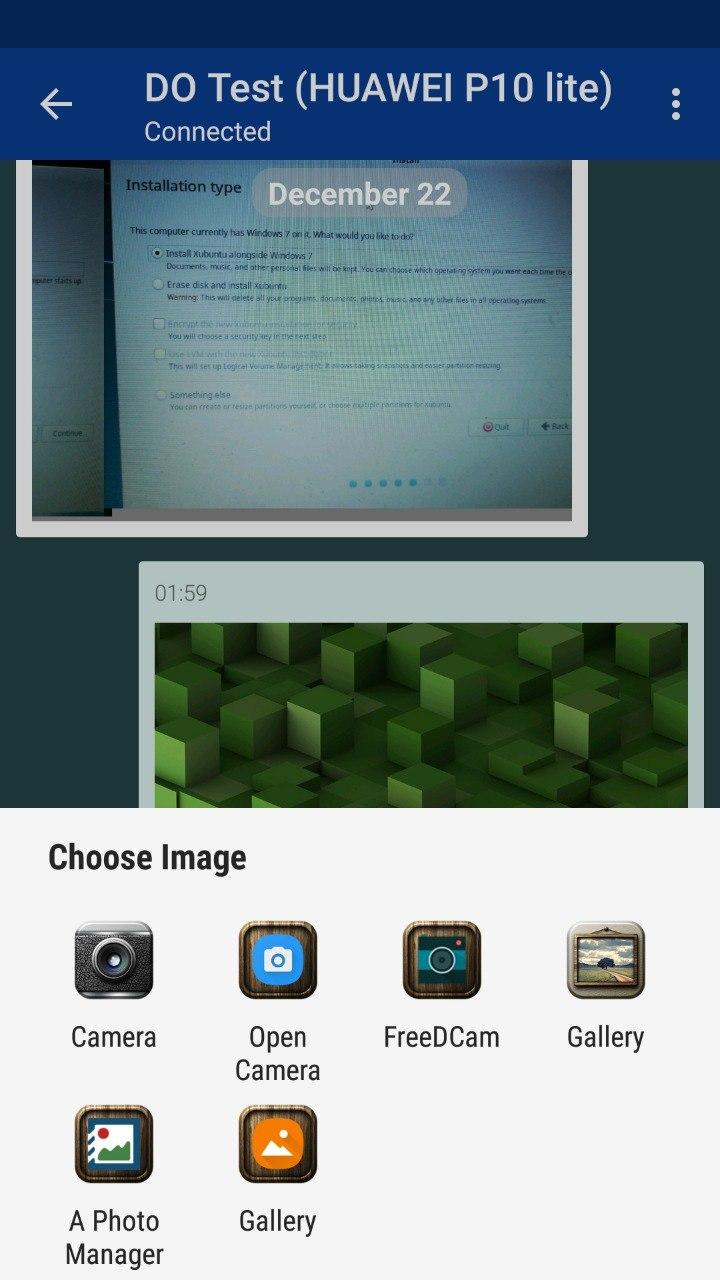
\includegraphics[width=0.8\textwidth]{chat_activity.jpg}}
		\label{fig:chat_activity}
		\caption{}
	\end{subfigure}
	\begin{subfigure}[t]{0.48\textwidth}
	    \centering                                                           
		\fbox{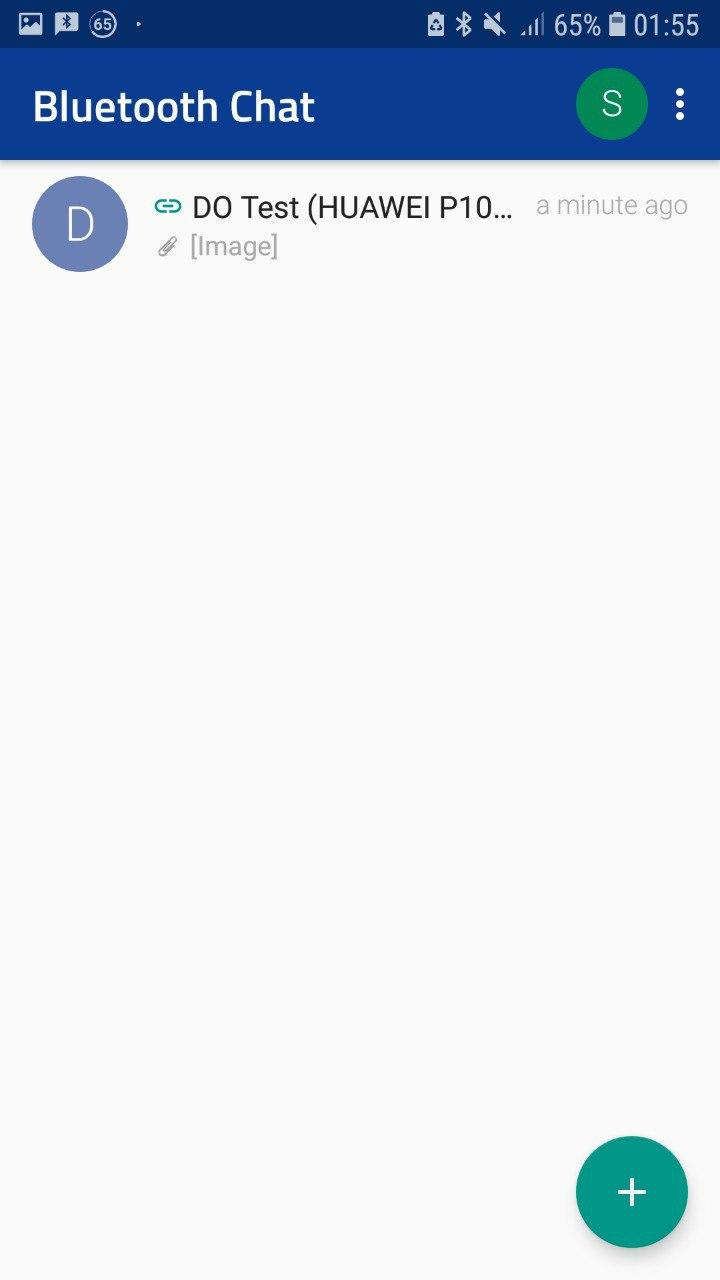
\includegraphics[width=0.8\textwidth]{conversations_activity.jpg}}
		\label{fig:conversations_activity}
		\caption{}
	\end{subfigure}
	\caption{Внешний вид экранов текущего чата и списка всех чатов}
	\label{fig:chat_and_conversations_activities}
\end{figure}

Экран текущего чата содержит сообщения, ранее отправленные данному пользователю, либо принятые от него; текстовое поле для ввода нового сообщения; также имеется кнопка, при нажатии на которую открывается меню выбора изображения, которое будет прикреплено в качестве вложения к очередному сообщению в текущем чате.

На рисунке \ref{fig:profile_and_receivied_images_activities}, а изображён внешний вид экрана профиля (появляется при первом запуске приложения). Экран профиля содержит содержит поле для ввода имени (под этим именем вы будете видны другим пользователям), кнопку выбора цвета фона изображения профиля (т. н. аватар), а также название устройства, заданное в системном меню настроек Bluetooth устройства.
На рисунке \ref{fig:profile_and_receivied_images_activities}, б представлен экран, содержащий список полученных изображений. Здесь отображаются все изображения, когда-либо полученные от других пользователей.
При нажатии на одно из изображений из списка, в правом верхнем углу экрана появляется значок удаления данного изображения.

\begin{figure}[ht]
	\centering
	\begin{subfigure}[t]{0.48\textwidth}
	    \centering                                                           
		\fbox{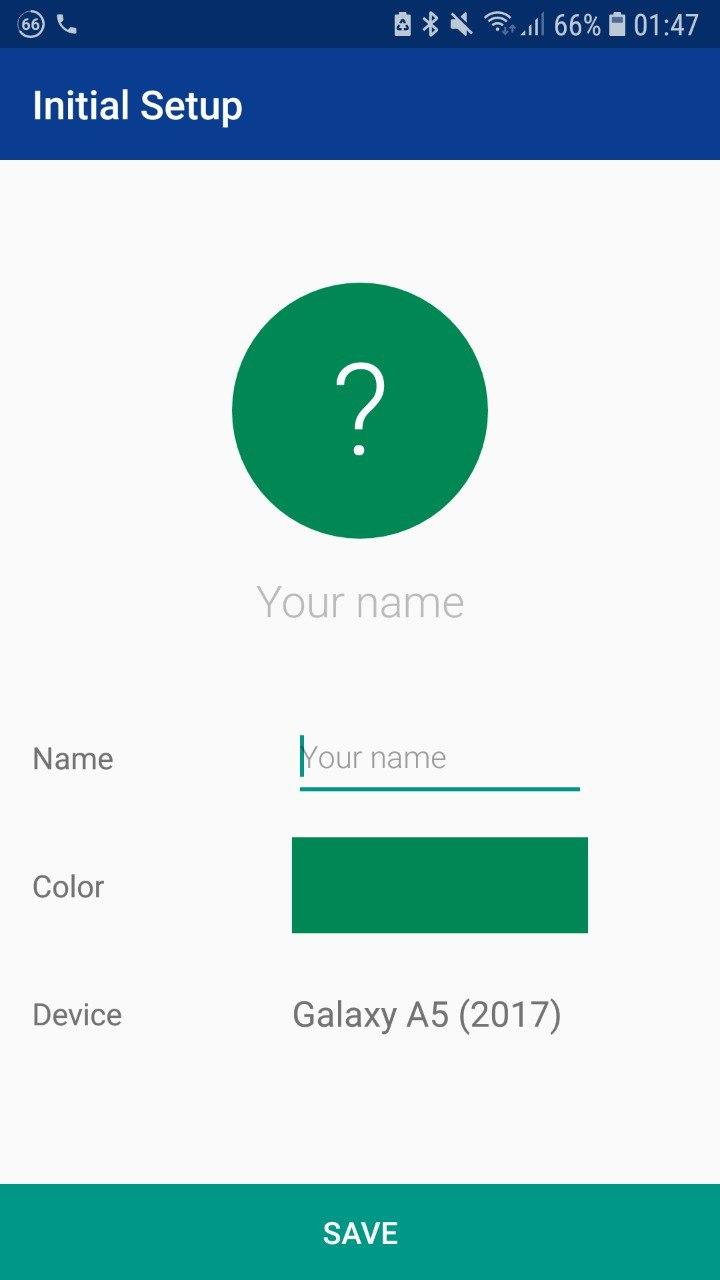
\includegraphics[width=0.8\textwidth]{profile_activity.jpg}}
		\label{fig:profile_activity}
		\caption{}
	\end{subfigure}
	\begin{subfigure}[t]{0.48\textwidth}
	    \centering                                                           
		\fbox{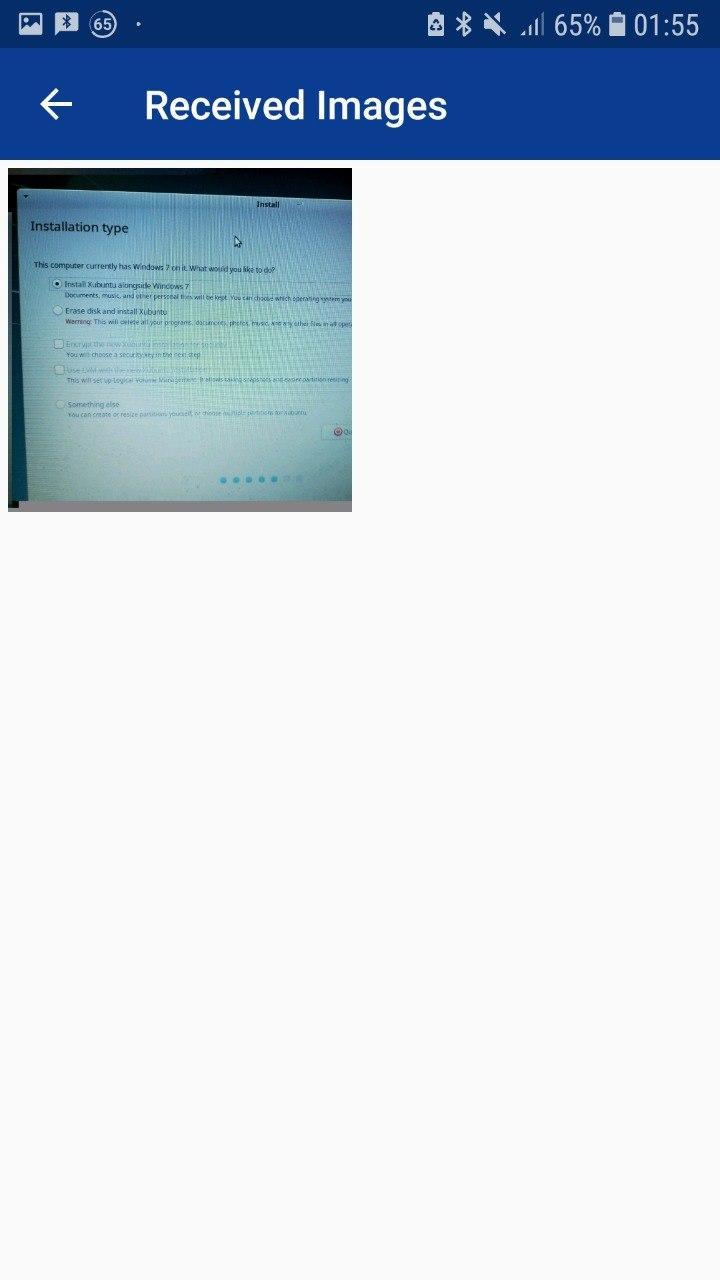
\includegraphics[width=0.8\textwidth]{received_images_activity.jpg}}
		\label{fig:received_images_activity}
		\caption{}
	\end{subfigure}
	\caption{Внешний вид экранов профиля и полученных изображений}
	\label{fig:profile_and_receivied_images_activities}
\end{figure}

На рисунке \ref{fig:scan_and_settings_activities}, а изображён внешний вид экрана сканирования устройств поблизости. На рисунке \ref{fig:scan_and_settings_activities}, б можно увидеть, как выглядит меню настроек разработанного приложения.

\begin{figure}[ht]
	\centering
	\begin{subfigure}[t]{0.48\textwidth}
	    \centering                                                           
		\fbox{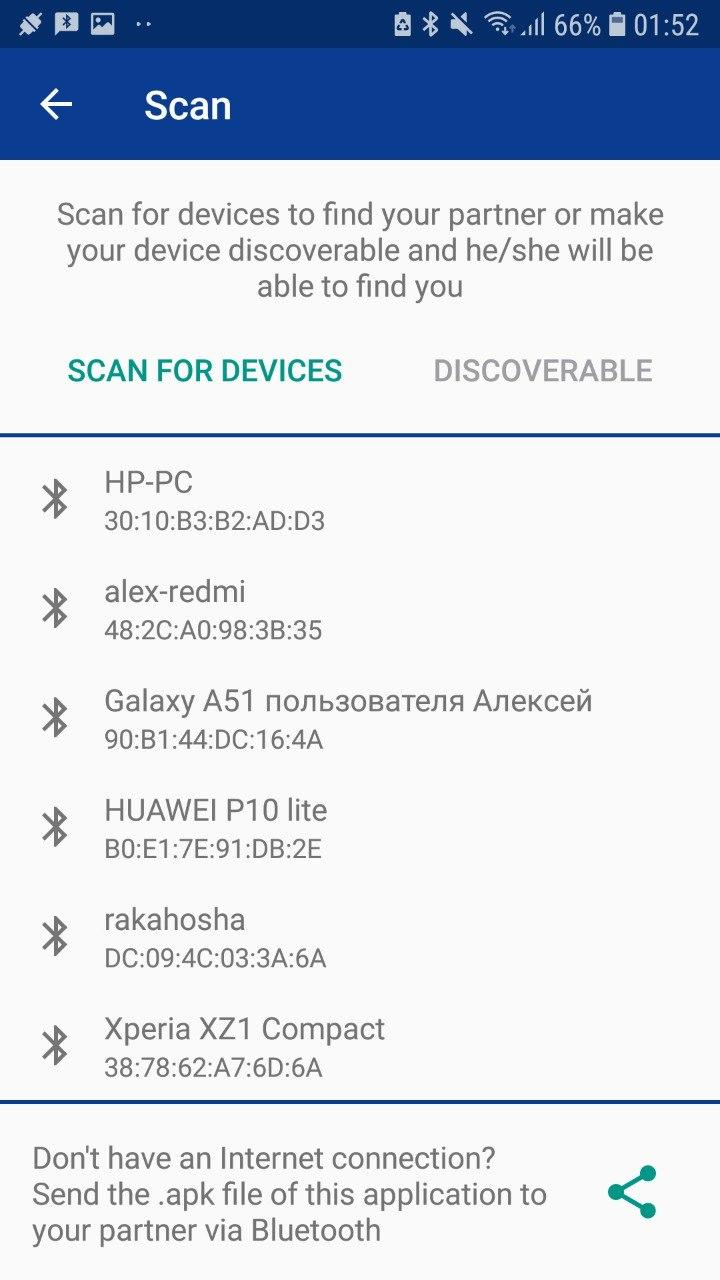
\includegraphics[width=0.8\textwidth]{scan_activity.jpg}}
		\label{fig:scan_activity}
		\caption{}
	\end{subfigure}
	\begin{subfigure}[t]{0.48\textwidth}
	    \centering                                                           
		\fbox{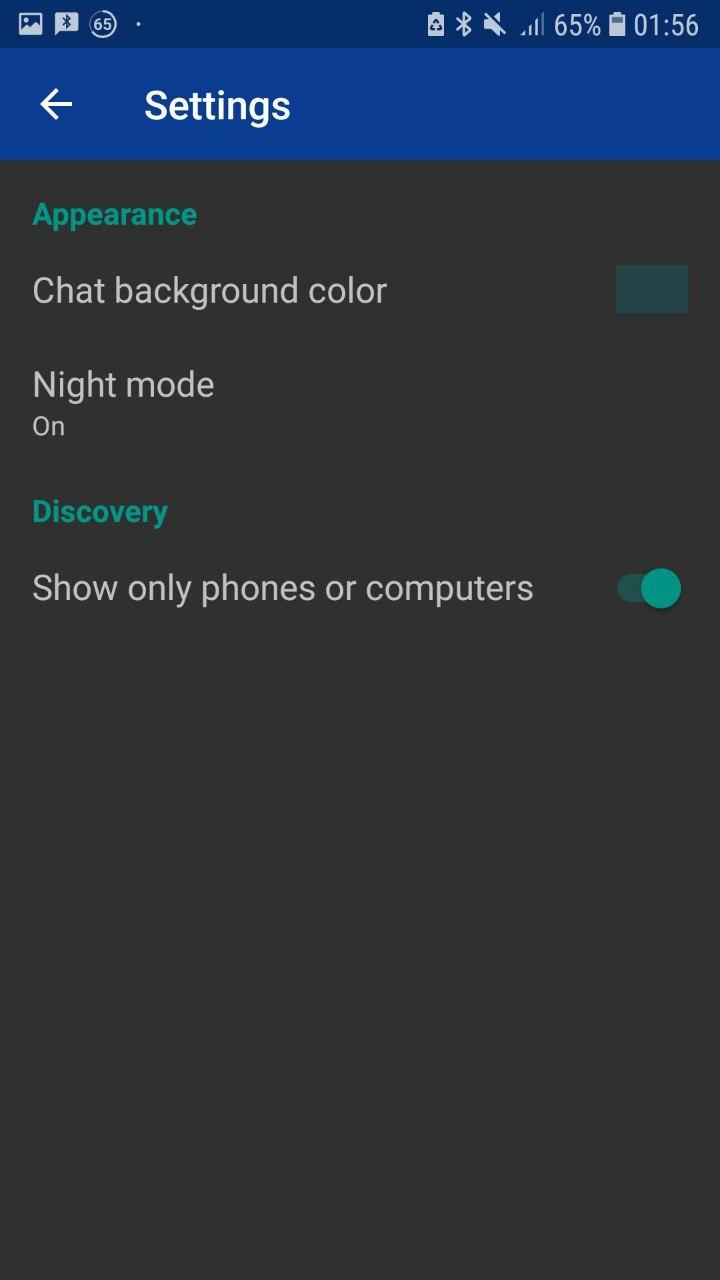
\includegraphics[width=0.8\textwidth]{settings_activity.jpg}}
		\label{fig:settings_activity}
		\caption{}
	\end{subfigure}
	\caption{Внешний вид экранов сканирования устройств и настроек}
	\label{fig:scan_and_settings_activities}
\end{figure}

На экране устройств поблизости представлены устройства, находящиеся рядом. Экран содержит кнопку перевода своего устройства в режим обнаружения на 300 секунд. Меню настроек содержит опции смены фона экрана чата, переключение темы между светлой и тёмной.
